\documentclass[11pt]{article}

\usepackage[utf8]{inputenc}
\usepackage{amsmath, amssymb, amsthm}
\usepackage[inkscapeformat=pdf]{svg}
\usepackage{placeins}
\usepackage{tabularx}
\usepackage{float}
\usepackage{setspace}
\usepackage{hyperref}
\usepackage{enumitem}
\usepackage{parskip}
\usepackage{ffcode}
\usepackage{graphicx}
\usepackage{caption}

\usepackage[margin=2cm]{geometry}

\usepackage{xcolor}
\definecolor{light-gray}{gray}{0.95}
\newcommand{\code}[1]{\colorbox{light-gray}{\texttt{#1}}}

\def\code#1{{\texttt{#1}}}

\title{%
  \textbf{IT} \\
  \large Software Engineering Project \\ A.Y. 2022-2023}

\author{Marco Ronzani, Alessandro Sassi}

\date{December 2022}

\begin{document}

\maketitle

\doublespacing
\tableofcontents
\singlespacing

\newpage

\section{Links to the software}

Follow the link to the source code and to a .README file that explains how to install and run the former.
\begin{itemize}
    \item \textbf{Source Code}: link here
    \item \textbf{Installation and usage instructions}: link here
\end{itemize}

\section{Introduction}
\label{section:introduction}

\subsection{Purpose}

Electric vehicles are starting to grow in number, and their takeover of combustion engines is bound to happen, consequently to support such a thriving trend adequate easy access to charging stations is of utmost importance. In this landscape the goal of eMall is to allow owners of electric vehicles to easily know where charging stations are and carefully plan their charging process according to their schedules at any such station. \\
\\
This document will follow up on the RASD and DD documents presenting the result of the development of a demonstrative viable prototype of the eMall software, please note that nice-to-have features have been disregarded when they were deemed not relevant to the overall functionalities to demonstrate. \\

\subsection{Scope}

This IT document start from what was layed down in the DD document and the requirements discussed in the RASD, presenting the result of the development of a prototype of eMall's software, complete with also the software of a CPO (a CPMS) which eMall relies upon to interact with CSs. Such software consists of a WebApp supported by a set of APIs which is itself reliant on APIs exposed by the software of CPMSs.

\subsection{Reference Documents}

\begin{enumerate}
    \item The provided document describing the project: \textit{Assignment IT AY 2022-2023}.
    \item The provided document describing the project: \textit{Assignment RDD AY 2022-2023-v3}.
    \item The Software Engineering 2 course held by Prof.s Camilli Matteo, Di Nitto Elisabetta and Rossi Matteo Giovanni.
    \item \textit{ISO/IEC/IEEE 29148:2011(E)} standard for Requirement Engineering.
    \item Project of last year provided as an assignment.
\end{enumerate}

\newpage

\section{Implemented Functionalities and Requirements}

The development of the prototype focused on the set of feature that were demanded in the first reference document for a group of two people.\\
Any requirement for which a justification is not provided regarding its exclusion from the prototype can be assumed to have been disregarded because outside of the following features \textit{(Those are marked with -)}.\\ \\
An eMSP shall offer to end users the possibility to:
\begin{enumerate}
    \item know about the charging stations nearby, their cost, any special offer they have.
    \item book a charge in a specific charging station for a certain time frame.
    \item start the charging process at a certain station.
    \item notify the user when the charging process is finished.
\end{enumerate}
A CPMS shall offer the following main functions:
\begin{enumerate}
    \item know the location and “external” status of a charging station (number of charging sockets available, their type such as slow/fast/rapid, their cost, and, if all sockets of a certain type are occupied, the estimated amount of time until the first socket of that type is freed).
    \item start charging a vehicle according to the amount of power supplied by the socket, and monitor the charging process to infer when the battery is full.
\end{enumerate}

\subsection{Functionalities}
Refer to the RASD document for detailed descriptions under section 2.2 .

\begin{table}[H]
    \centering
    %space between text and right/left borders
    \setlength{\tabcolsep}{18pt}
    %Row height multiplier
    \renewcommand{\arraystretch}{1.2}
    \begin{tabularx}{\textwidth}{|>{\centering\hsize=0.15\hsize}X|>{\hsize=1.425\hsize}X|>{\hsize=1.425\hsize}X|}
        \hline
        \textbf{Id} & \textbf{Functionality} & \textbf{Status} \\
        \hline
        1 & User registration & Implemented \\
        \hline
        1 & Search for CSs & Implemented \\
        \hline
        1 & Book a recharge at a CS & Implemented \\
        \hline
        1 & Perform a recharge at a CS & Implemented (mocked CS) \\
        \hline
        1 & Acquire price and energy mix information from DSOs & - \\
        \hline
        1 & Choose prices, energy sources and battery usage policies for a CS & - \\
        \hline
        1 & Allow the CPMS to operate automatically & - \\
        \hline
        1 & Allow the CPO to change the “Automatic Mode” policy used by the CPMS & - \\
        \hline
    \end{tabularx}
    \label{tab:requirements}
\end{table}

\subsection{Requirements}
Refer to the DD document for detailed descriptions under section 4 .

\begin{table}[H]
    \centering
    %space between text and right/left borders
    \setlength{\tabcolsep}{18pt}
    %Row height multiplier
    \renewcommand{\arraystretch}{1.2}
    \begin{tabularx}{\textwidth}{|>{\centering\hsize=0.15\hsize}X|>{\hsize=1.425\hsize}X|>{\hsize=1.425\hsize}X|}
        \hline
        \textbf{Id} & \textbf{Requirement} & \textbf{Status} \\
        \hline
        R1 & The eMSP shall allow a registered user to login & Implemented \\
        \hline
        R2 & The eMSP shall allow an unregistered user to register on the platform & Implemented \\
        \hline
        R3 & The eMSP should report to the user when they sent invalid input data through a form & Implemented \\
        \hline
        R4 & The eMSP should report to the user when they attempted to perform an unauthorized action & Implemented \\
        \hline
        R5 & The eMSP should report to the user when the platform encountered an error while processing the action & Implemented \\
        \hline
        R6 & The eMSP should report to the user any successful action performed & Implemented \\
        \hline
        R7 & The eMSP shall allow a logged-in user to view charging stations nearby & Implemented \\
        \hline
        R8 & The eMSP shall allow a logged-in user to know the cost of a recharge at a CS & Implemented \\
        \hline
        R9 & The eMSP shall allow a logged-in user to know about ongoing special offers present at a CS & Implemented \\
        \hline
        R10 & The eMSP shall allow a logged-in user to book a recharge at a free socket of a CS for a given time slot & Implemented \\
        \hline
        R11 & The eMSP shall allow a logged-in user to cancel any of its booked recharges before their scheduled time & Implemented \\
        \hline
        R12 & The eMSP shall not allow a user to book a recharge at a socket of a CS which has already been booked for the chosen time slot & Implemented \\
        \hline
        R13 & The eMSP shall not allow a user to book multiple recharges with overlapping time slots & Implemented \\
        \hline
        R14 & The eMSP shall allow a logged-in user to see their bookings & Implemented \\
        \hline
        R15 & The eMSP shall allow a logged-in user to start the charging process for one of their booked recharges & Implemented \\
        \hline
        R16 & The eMSP shall not allow a user without a booking to start the charging process & Implemented \\
        \hline
    \end{tabularx}
    \label{tab:requirements}
\end{table}

\begin{table}[H]
    \centering
    %space between text and right/left borders
    \setlength{\tabcolsep}{18pt}
    %Row height multiplier
    \renewcommand{\arraystretch}{1.2}
    \begin{tabularx}{\textwidth}{|>{\centering\hsize=0.15\hsize}X|>{\hsize=1.425\hsize}X|>{\hsize=1.425\hsize}X|}
        \hline
        \textbf{Id} & \textbf{Requirement} & \textbf{Status} \\
        \hline
        R17 & The eMSP shall not allow a user to start the charging process as long as the socket is vacant & Implemented \\
        \hline
        R18 & The eMSP should notify a logged-in user when their ongoing charging processes is complete & Implemented \\
        \hline
        R19 & The eMSP should notify a logged-in user when their ongoing charging process is terminated due to the expiration of its booked time slot & Implemented \\
        \hline
        R20 & The eMSP shall allow a logged-in user to terminate their charging process earlier & Implemented \\
        \hline
        R21 & The eMSP should charge a user for everyone of his charging processes as soon as they finish & Implemented (mockup) \\
        \hline
        R22 & The eMSP shall charge a user for a fee if they do not start a recharge during their booking's time slot & - \\
        \hline
        R23 & The eMSP shall be able to offer its functionalities to multiple users at once & eMSP: Implemented \\
        \hline
        R24 & The CPMS should be able to acquire the location from CSs & Implemented (mocked via a fake CS client, with the data present anyway in teh CPMS's DB) \\
        \hline
        R25 & The CPMS should be able to acquire the internal status from CSs & - \\
        \hline
        R26 & The CPMS should be able to acquire the external status from CSs & Implemented \\
        \hline
        R27 & The CPMS should be able to start charging a vehicle connected to a CS socket & Implemented (mocked via a fake CS client) \\
        \hline
        R28 & The CPMS should be able to monitor the charging process of a vehicle & Implemented (mocked via a fake CS client) \\
        \hline
        R29 & The CPMS should be able to acquire from DSOs their current energy prices & - \\
        \hline
        R30 & The CPMS should be able to acquire from DSOs their energy mix & - \\
        \hline
        R31 & The CPMS shall allow its CPO to authenticate with it & - \\
        \hline
        R32 & The CPMS shall allow its CPO to assign a DSO to a CS as its energy provider  when operating in “Manual Mode” & - \\
        \hline
    \end{tabularx}
    \label{tab:requirements}
\end{table}

\begin{table}[H]
    \centering
    %space between text and right/left borders
    \setlength{\tabcolsep}{18pt}
    %Row height multiplier
    \renewcommand{\arraystretch}{1.2}
    \begin{tabularx}{\textwidth}{|>{\centering\hsize=0.15\hsize}X|>{\hsize=1.425\hsize}X|>{\hsize=1.425\hsize}X|}
        \hline
        \textbf{Id} & \textbf{Requirement} & \textbf{Status} \\
        \hline
        R33 & The CPMS should be able to automatically assign a DSO to a CS as its energy provider when operating in “Automatic Mode” & - \\
        \hline
        R34 & The CPMS shall allow the CPO to decide the energy source management policies when operating in “Manual Mode” & - \\
        \hline
        R35 & The CPMS should be able to automatically choose the current energy source for a CS according to the given policy when operating in “Automatic Mode” & - \\
        \hline
        R36 & The CPMS shall allow its CPO to assign a nominal-price, a user-price and an offer reset date to a CS when operating in “Manual Mode” & - \\
        \hline
        R37 & The CPMS should be able to automatically assign a nominal-price, a user-price and an offer reset to a CS when operating in “Automatic Mode” & - \\
        \hline
        R38 & The CPMS shall allow the CPO to choose its policy for operating in “Automatic Mode” & - \\
        \hline
        R39 & The CPMS shall allow the CPO to choose whether it acts automatically or manually & - \\
        \hline
        R40 & The CPMS shall never take a decision automatically when it is set in “Manual Mode” & - \\
        \hline
        R41 & The CPMS should report to the user when they sent invalid input data & Implemented \\
        \hline
        R42 & The CPMS should report to the user when they attempted to perform an unauthorized action & Implemented \\
        \hline
        R43 & The CPMS should report to the user when the platform encountered an error while processing the action & Implemented \\
        \hline
        R44 & The CPMS should be able to decide whether to start charging the internal batteries of a CS (if present) & - \\
        \hline
    \end{tabularx}
    \label{tab:requirements-2}
\end{table}

\newpage

\section{Adopted development frameworks}

As expected of every modern Web Application supported by a backend API, its software architecture is divided in a Model and Routes for the backend and a framework for the frontend which allows for both a logic and presentation layer in order to offer more advanced functionalities that a plain HTTP page. \\
In the prototype here discussed keep in mind that there is a further distinction between the CPMS's backend and the eMSP's one, when neither is mentioned explicitly, what follows refers to both.

\subsection{Adopted programming languages}

\subsubsection{TypeScript}

Both backends and the frontend are primarily written in \textbf{TypeScript}, a superset of Javascript that adds to the former static typing and optional classes and interfaces, resulting in better type safety and less mandelbugs. TypesScript unfortunately offers a considerably smaller set of libraries compared to JavaScript, but nonetheless did not hinder the capabilities of the final prototype.

\subsubsection{SQL}

The interactions with the database that occur within the model are realized by preparing and executing SQL statements, such queries make extensive use of MySQL's dialect of SQL, requiring no redundant storage of data on the database and a simple way to recover from it only what is necessary.

\subsubsection{HTML and CSS}

%TODO

\subsection{Adopted middleware}

\subsubsection{Express.js as a Request Router for the backend}

Express is a free and open-source web framework for building APIs with a comprehensive set of features. Its approach to middleware and routing, which involves adding functions to endpoint declarations, helps improve code scalability. The use of functions as middleware also promotes modularity in the application by allowing endpoints to be added through corresponding functions for each route.

\subsubsection{Database connection with MySQL2}

MySQL is a set of modules for working with the MySQL database, it is a typescript version of the popular MySQL package. This library was chosen for its excellent pooling system and the possibility of preparing statements before executing queries, where the query string is passed directly to the database and parameters are replaced there, preventing the risk of SQL injection that can result from string concatenation on the server.

\subsubsection{Connection to the CS via WebSocket}

The WebSocket library for JavaScript (ws) enables real-time, two-way communication between a client and a server, it provides a simple and efficient API for creating and managing connections, supporting both server-side and client-side use.

\subsubsection{Http requests via the Axios library}

Axios is JavaScript library for making HTTP requests in Node.js, it is promise-based and enables sending HTTP requests to access REST APIs and other web services. Axios abstracts away some of the complexities of making HTTP requests and provides a simple, straightforward API for handling requests and responses.

\subsection{Utilized APIs (not present in the DD)}

%maybe Google Maps here?

\subsection{Platforms and Libraries}

\subsubsection{Node.js}

Node is an open-source, cross-platform, back-end JavaScript (and by extension TypeScript) runtime environment which offers many stable and well known libraries (ex: Express). It allows the execution of JavaScript outside of a web browser and as act as a server, is well-suited for building responsive applications, such as eMall, due to its ability to handle multiple simultaneous connections with low latency. Its only drawback is its single-threaded model, resulting in poor performances when dealing with CPU-intensive tasks, but that is never the case with the present prototype.

\subsubsection{Authentication with JWT and BCrypt}

JWT (JSON Web Token) is a javascript implementation of the JSON Web Token standard, which provides a secure and URL-safe method of transferring user information between two parties. \\
\\
BCrypt is the Javascript implementation of the bcrypt hashing function based, a standard to hide passwords in a web environment. It provides a simple and secure way to hash passwords and compare them during authentication.

\subsubsection{Testing with Mocha and Sinon-Chai}

Mocha is a JavaScript testing framework that works with Node.js. It provides a simple, flexible, and fast environment for writing and executing test cases for applications and libraries. \\
Sinon-Chai is comprised of the two libraries Sinon and Chai, the first allows for testing via stubs and mocks of objects and functions, the second complements it with an easy way to write assertions.

\subsubsection{Frontend with Vue}

%TODO

\section{Source code structure}

As mentioned in the DD document, the structure of the code is made to reflect the Model View Controller (MVC) pattern. Briefly: \\
\begin{itemize}
    \item \textbf{Model}, it contains the logic that retrieves from the database the data that needs to be show to the user, as well as classes used to incapsulate the data retrieved. Ad-hoc versions of the model exist for the frontend and backend. \\
    More precisely there are 3 different models, one for the eMSP's backend, one for its frontend, and one for the CPMS's backend.
    \item \textbf{View}, its goal is to show the data of the model to the user, formatted in a human-friendly way. The view is realized with the above-mentioned Vue framework and is present only for the eMSP.
    \item \textbf{Controller}, logic in charge of using the Model to feed the View and respond to user inputs, it is comprised of the client-side modules used to asynchronously request and send data to the backend, but also the Server-side components handling all API routes.
\end{itemize}

Reflecting such structure is the hierarchy of directories within the source code, atleast for what concerns the backend of the CPMS and eMSP, with the added paths being for tests and helper functions:
\begin{itemize}
    \item \textit{src/routes} are the express routes realizing the aforementioned controller.
    \item \textit{src/model} contains all the classes for data representation and retrieval from the database.
    \item \textit{src/test} contains, following the same hierarchy as the \textbf{src} directory, the tests for the entire backend.
    \item \textit{src/helper} consists of some miscellaneous utility functions, each commented in detail.
\end{itemize}

The frontend follows the a structure not so different from the two backends, with the notable additions of:
\begin{itemize}
    \item \textit{src/components} stores Vue components, which are reusable user interface elements.
    \item \textit{src/controllers}, contains JavaScript files that define the behavior and logic of the web application, interacting with the Vue instance and the backend.
    \item \textit{src/views} contains components that define the layout and structure of the frontend's web pages, those define the application's routing as well.
\end{itemize}

Refer to the DD for an overview of the modules involved.\\
\\
The only module present, not previously discussed as such in the DD is the "bank" module, which simply simulates the "payment provider" mentioned in the DD, hence refer to the latter.

\newpage

\section{Testing}

See the DD for a more detailed description of the following process.

\subsection{Integration testing}

Following what was discussed in the DD document, integration testing has been performed during each phase of the development, which proceeded in parallel for both the CPMS and eMSP backends, with their final integration with one-another occurring only when both were already fully ready. \\
Internally each backend had its development start from the database, then data access modules (the previously discussed Models) followed by the rest of the control logic (the Routes). After the routes went through testing and were complemented with the authentication capabilities the final set of integration test could be done, before moving on to the frontend development and finally full integration tests. \\
\\
In more detail every module's API has been tested with PostMan (\href{https://www.postman.com/}{https://www.postman.com/}) and MySQL WorkBench (\href{https://www.mysql.com/products/workbench/}{https://www.mysql.com/products/workbench/}), in order:

\begin{enumerate}
    \item After constructing of each module's database and Model, the utilized queries were tested with MySQL WorkBench by:
    \begin{itemize}
        \item Running the queries directly from WorkBench, with dummy DB entries and query parameters.
        \item Running the queries from the Model, ran withing Node,js, using dummy mains, follows an example of such tests for the "CS.ts" model file within the CPMS's backend: \\
        \code{CS.getCSList([30, 140], 20, [2, 20]).then(
                async (result) => \{
                console.log(result); \\
            await DBAccess.closePool();\}} \\
            This has been done together with active logging within the database instance to ensure the correct format of parameters inserted into prepared statements: \\
        \code{SET GLOBAL log\_output = 'TABLE';\\
                SET GLOBAL general\_log = 'ON';\\
                SELECT * FROM mysql.general\_log;}
    \end{itemize}
    
    \item Each realized API interface has been tested during and after construction, together with the Model it relied upon, with PostMan, by sending to it HTTP requests and verifying both the correctness of responses and the tolerance of the API to malformed requests. Follow some examples of the performed tests:
    
    \newpage
    
    \begin{figure}[!ht]
        \centering
        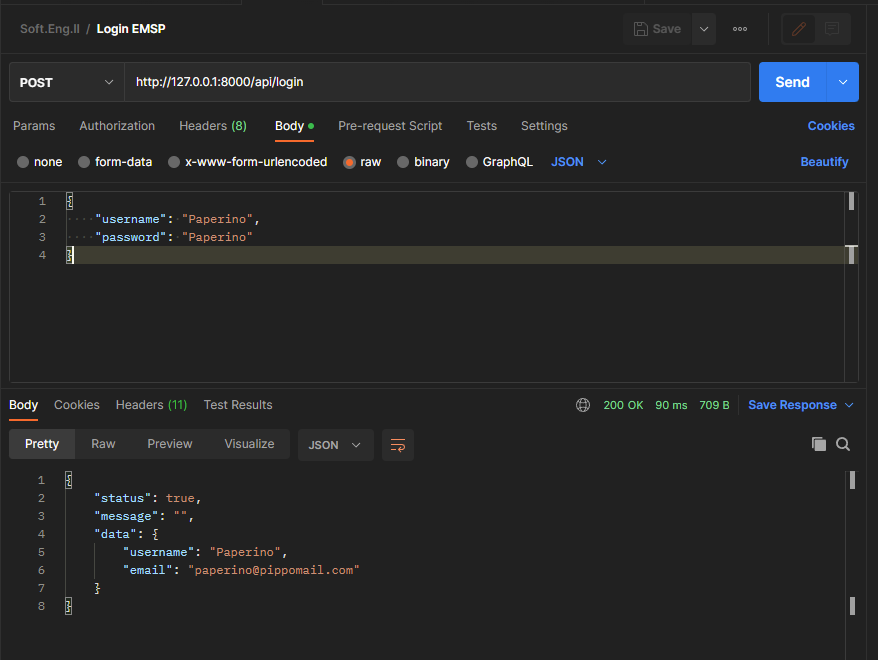
\includegraphics[width=130mm]{LoginEMSP.PNG}
        \captionsetup{justification=centering,margin=2cm}
        \caption{Testing of the EMSP Login endpoint, resulting in a success}
        \label{fig:my_label}
    \end{figure}
    
    \begin{figure}[!ht]
        \centering
        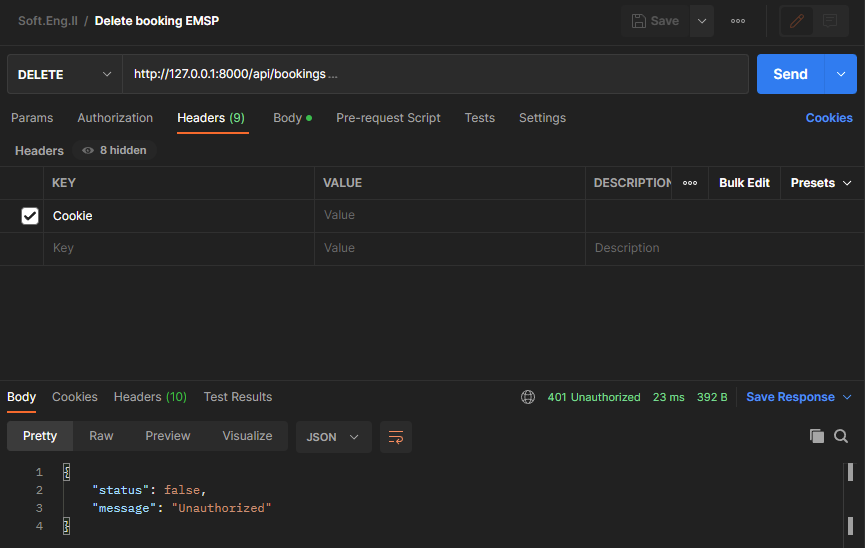
\includegraphics[width=130mm]{DeleteBookingFail.PNG}
        \captionsetup{justification=centering,margin=2cm}
        \caption{Testing of the EMSP Bookings endpoint, a attempt to access any booking before being logged in fails}
        \label{fig:my_label}
    \end{figure}
    
    \newpage

    \begin{figure}[!ht]
        \centering
        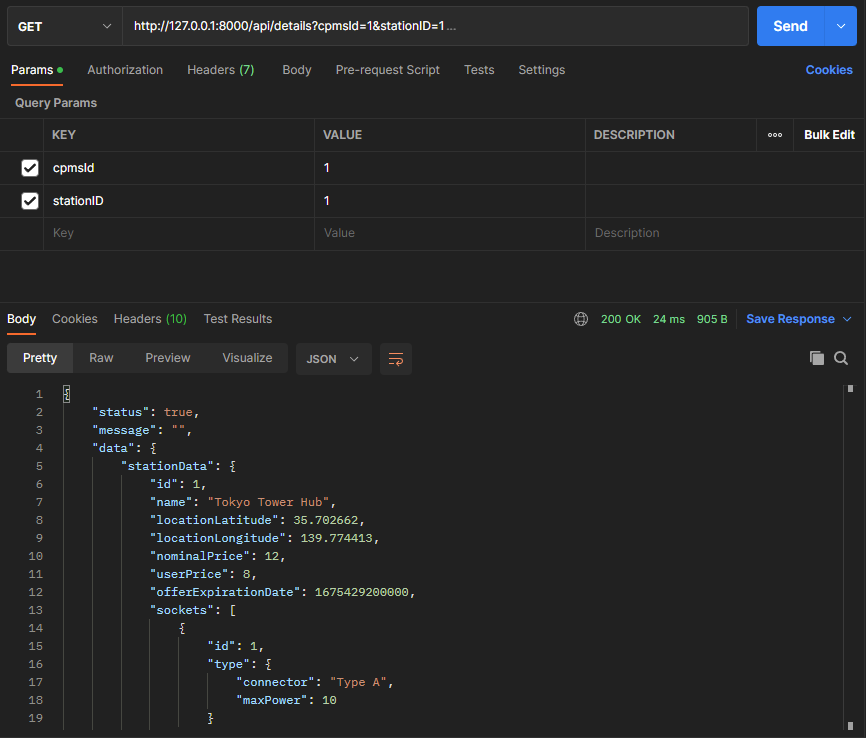
\includegraphics[width=110mm]{CSDetails.PNG}
        \captionsetup{justification=centering,margin=2cm}
        \caption{Testing of the EMSP Details endpoint, a logged in user received an object describing the requested CS}
        \label{fig:my_label}
    \end{figure}
    
    \begin{figure}[!ht]
        \centering
        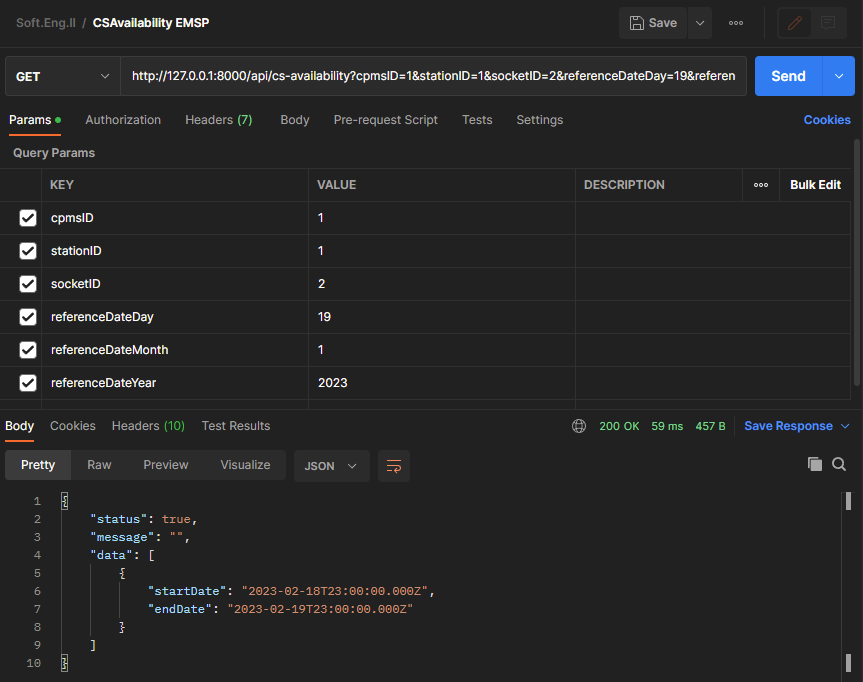
\includegraphics[width=110mm]{Availability.PNG}
        \captionsetup{justification=centering,margin=2cm}
        \caption{Testing of the EMSP Availability endpoint, it correctly responds to a logged in user with the intervals in which the specified CS is available for the provided date}
        \label{fig:my_label}
    \end{figure}
    
    \newpage
    
    \begin{figure}[!ht]
        \centering
        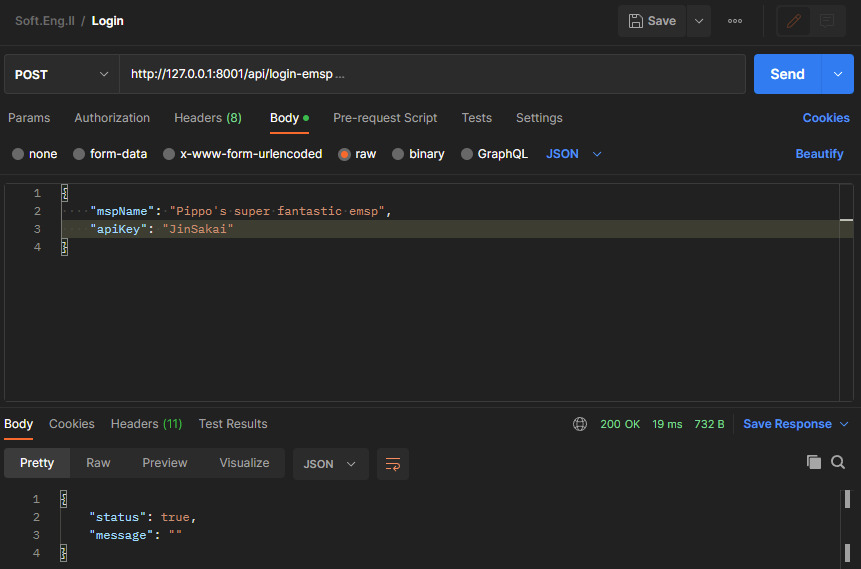
\includegraphics[width=120mm]{LoginCPMS.PNG}
        \captionsetup{justification=centering,margin=2cm}
        \caption{Testing of the CPMS Login-emsp endpoint, resulting in a success}
        \label{fig:my_label}
    \end{figure}
    
    \begin{figure}[!ht]
        \centering
        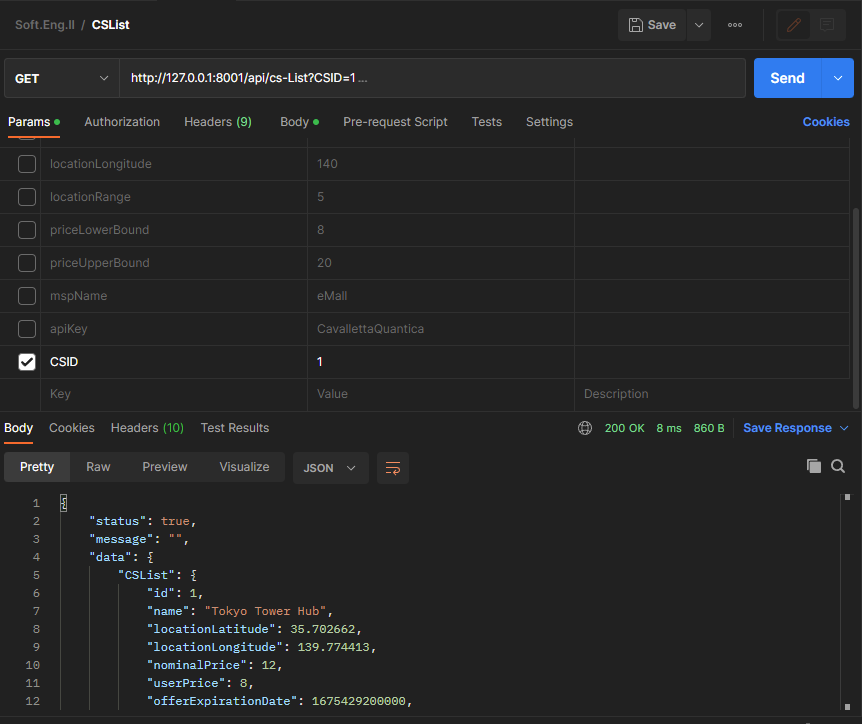
\includegraphics[width=120mm]{CSList.PNG}
        \captionsetup{justification=centering,margin=2cm}
        \caption{Testing of the CPMS CS-list endpoint, that returns to an authenticated EMSP a filtered list of charging stations information}
        \label{fig:my_label}
    \end{figure}
    
\end{enumerate}

\newpage

\subsection{Automated testing}

Automated tests have been written for every route with the aid of Sinon-Chai, during those tests the interactions with the database are always stubbed with SinonStub instances that replace every connections to the DB, returning predefined results that consequently not only test the behaviour of the routes, but of the Model as well.
Every route of the CPMS and EMSP has been fully tested, no tests are present for the bank as it is just a mockup. \\
\\
To run the tests, assuming that you already followed the \textbf{Installation instructions} in the section below, you can follow those instructions:
\begin{enumerate}
    \item \textbf{Run the CPMS's tests} by reaching its location, \code{YourProjectRoot/cpms/backend}, with a console and running the command: \code{npm run test}.
    \item \textbf{Run the eMSP's tests} by reaching its location, \code{YourProjectRoot/emsp/backend}, with a console and running the command: \code{npm run test}.
\end{enumerate}
You can also produce coverage reports (an pre-evaluated instance is already included in the project) with the following commands:
\begin{enumerate}
    \item \textbf{Evaluate the CPMS's coverage} by reaching its location, \code{YourProjectRoot/cpms/backend}, with a console and running the command: \code{npm run coverage}.
    \item \textbf{Evaluate the eMSP's coverage} by reaching its location, \code{YourProjectRoot/emsp/backend}, with a console and running the command: \code{npm run coverage}.
\end{enumerate}
The coverage reports can be view by opening \code{YourProjectRoot/cpms/backend/coverage/index.html} and \code{YourProjectRoot/emsp/backend/coverage/index.html}.
At the time of writing the coverage results are as follow:

\begin{figure}[!ht]
    \centering
    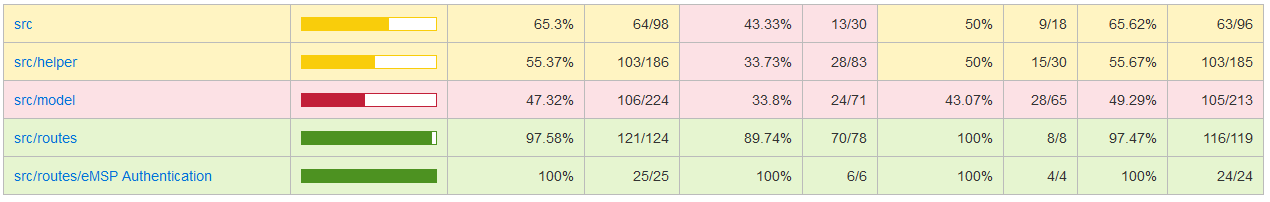
\includegraphics[width=160mm]{CPMSCoverage.PNG}
    \captionsetup{justification=centering,margin=2cm}
    \caption{Coverage of the CPMS}
    \label{fig:my_label}
\end{figure}

\begin{figure}[!ht]
    \centering
    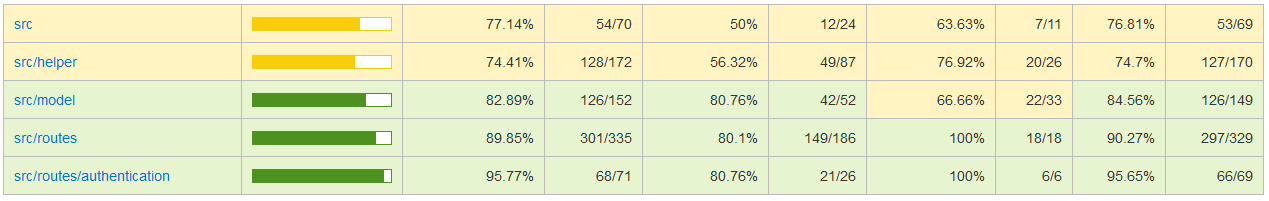
\includegraphics[width=160mm]{EMSPCoverage.PNG}
    \captionsetup{justification=centering,margin=2cm}
    \caption{Coverage of the EMSP}
    \label{fig:my_label}
\end{figure}

Note that the coverage of the CPMS could not be improved due to the presence of the charging station mockup and its materialization in the CPMS's backend, CSConnection, both of which cannot be tested due to their complete reliance on WebSockets and a live connection for their functionalities, hence any test would have just consisted of stubs interacting with one-another.

\newpage

\section{Installation instructions}

\subsection{Prerequisites}

\begin{itemize}
    \item \textbf{MySQL Server} is required to be installed on your system, download it from here: \\ \href{https://dev.mysql.com/downloads/installer/}{https://dev.mysql.com/downloads/installer/}. \\
    For installations on Windows you can refer to this guide: \\ \href{https://dev.mysql.com/doc/refman/8.0/en/windows-installation.html}{https://dev.mysql.com/doc/refman/8.0/en/windows-installation.html}. \\
    Ensure to take note of your root password during installation, it will be usefull later.
    
    \item \textbf{MySQL WorkBench} is not necessary, but recommended to allow you to import the provided database dump into your instance of MySQL Server. You can download it from here: \\
    \href{https://dev.mysql.com/downloads/workbench/}{https://dev.mysql.com/downloads/workbench/} \\
    After installing WorkBench, connect it to your local instance of MySQL Server (which must be up and running for this to work), first choose to create a new connection (+ button near "My Connections"), then set its host to "localhost" and port to "3306". Your username for the connection is recommended to be "root", and its password the one chosen during the installation of MySQL Server. Note that you can use other user accounts as long as you give them high enough privileges to import a schema and operate on it at will.
    
    \item \textbf{Node.js} must be present on your system, only version 18.12.0 was tested, you can download it from here: \\
    \href{https://nodejs.org/download/release/v18.12.0/}{https://nodejs.org/download/release/v18.12.0/} \\
    The installation is guided and simple. Ensure node is present in your system path.
\end{itemize}

\subsection{Preparing the Project}

\begin{enumerate}
    \item \textbf{Download the Project} download the ".zip" file provided with the project (It is located under "/DeliveryFolder" on GitHub) and extract it in a known location.
    \item \textbf{Import the schemas in the DB} by opening MySQL Workbench and opening the DB connection you previously configured, in the left-side menu select "Administration" and then "Import Data/Restore". The screen to import database dumps will open and you will need to select "Import from Self-Contained File" and choose as the file to import \code{YourProjectRoot/DBs\_dump.sql}, and then choose to "Start the Import". \\
    This will create in your MySQL local instance of the \code{emsp\_db}, \code{cpms\_db} and \code{bank\_db} schemas. \\
    If you can't access the newly imported schemas after "Schemas" on the left menu, close and reopen WorkBench.
    \item \textbf{Run NPM} to download all the node packages required for the project, to do this open a terminal and reach each of the following paths within the extracted project folder, in each path run: \code{npm install} \\
    List of paths:
    \begin{itemize}
        \item \code{YourProjectRoot/cpms/backend}
        \item \code{YourProjectRoot/emsp/backend}
        \item \code{YourProjectRoot/emsp/frontend}
    \end{itemize}
    This should fetch all node modules listed in "package.json" for each of the 3 directories containing the CPMS's backend, the eMSP's backend and the eMSP's frontend.
    \item \textbf{Configure the ".env" files}, there are 2 ".env" files you need to configure to reflect your MySQL installation, they are located in:
    \begin{itemize}
        \item \code{YourProjectRoot/cpms/backend}
        \item \code{YourProjectRoot/emsp/backend}
    \end{itemize}
    The only needed change is to the field "DB\_PASSWORD", which should be set to the root password you chose while installing MySQL Server. \\
    If you also are using a different user than "root", you can account for it by changing the "DB\_HOST" accordingly field too. \\
    Note: not quotes required.
\end{enumerate}

\subsection{Running the project}

Run each of the following programs, in the specified order (not a must, but highly suggested).

\begin{enumerate}
    \item \textbf{Run the CPMS's backend} by reaching its location, \code{YourProjectRoot/cpms/backend}, with a console and running the command: \code{npm run run}.
    \item \textbf{Run the CS mockup}, for any CS you wish to emulate of the 9 available ones, by reaching its location, \code{YourProjectRoot/cpms/backend}, with a console and running the command: \\ \code{npm run run-cs [ID]}, where "ID" is a number from 1 to 9 (extremes included) indicating the charging station ID. Refer to the following figure for which id is of which charging station.
    
    \begin{figure}[!ht]
        \centering
        \includegraphics[width=160mm]{css.jpg}
    \end{figure}
    
    You can run multiple mockups by opening multiple console instances and repeating the above procedure, however do not run two mockups on the same charging station ID.
    
    \item \textbf{Run the bank's backend} by reaching its location, \code{YourProjectRoot/bank/backend}, with a console and running the command: \code{npm run run}.
    \item \textbf{Run the eMSP's backend} by reaching its location, \code{YourProjectRoot/emsp/backend}, with a console and running the command: \code{npm run run}.
    \item \textbf{Run the eMSP's frontend} by reaching its location, \code{YourProjectRoot/emsp/frontend}, with a console and running the command: \code{npm run dev}.
\end{enumerate}

\subsection{Intercting with the running project}

\begin{enumerate}
    \item \textbf{Reach the WebApp} by opening the URL printed during the frontend's startup, which should be \code{\href{http://localhost:5173/}{http://localhost:5173/}}.
    \item \textbf{Manually operate the CS mockup} by utilizing the following commands:
    \begin{itemize}
        \item \code{connectCar [socketId]} : simulates a car connecting to the given socket.
        \item \code{disconnectCar [socketId]} : simulates a car disconnecting from the given socket.
        \item \code{fullyCharge [socketId]} : simulates a car charging completely over the given socket.
        \item \code{quit} : closes the program.
        \item \code{help} : to print those instructions in the program.
    \end{itemize}
\end{enumerate}

\section{Effort Spent}

\subsection{Ronzani Marco - mat: 224578}

\begin{tabular}{|l|l|}
    \hline
    \textbf{Task} & \textbf{Time spent} \\
    \hline
    Backend (APIs and Models) & $25 h$ \\
    \hline
    Frontend & $0 h$ \\
    \hline
    Tests & $16 h$ \\
    \hline
    Documentation & $4 h$ \\
    \hline
    This document & $4 h$ \\
    \hline
    \hline
    Total & $49 h$ \\
    \hline
\end{tabular}

\subsection{Sassi Alessandro - mat: 220837}

\begin{tabular}{|l|l|}
    \hline
    \textbf{Task} & \textbf{Time spent} \\
    \hline
    Backend (APIs and Models) & $x h$ \\
    \hline
    Frontend & $x h$ \\
    \hline
    Tests & $x h$ \\
    \hline
    Documentation & $x h$ \\
    \hline
    This document & $x h$ \\
    \hline
    \hline
    Total & $x h$ \\
    \hline
\end{tabular}

\newpage

\section{References}
\label{section:references}

\begin{enumerate}
    \item \href{https://www.chargelab.co/}{ChargeLab - operating system for EV charges}
    \item \href{https://www.platformelectromobility.eu/2022/05/17/ev-charging-how-to-tap-in-the-grid-smartly/}{Platform for Electromobility. EV Charging: How to tap in the grid smartly?}.
    \item \href{https://mobilityintegrationsymposium.org/wp-content/uploads/sites/10/2018/11/4A_3_Emob18_024_paper_Filipe_Campos.pdf}{F. Campos, L. Marques, and K. Kotsalos, Electric Vehicle CPMS and Secondary Substation Management}.
    \item \href{https://doi.org/10.1145/3297067.3297078}{Shu Su, Hui Yan, and Ning Ding. 2018. Machine Learning-Based Charging Network Operation Service Platform Reservation Charging Service System. In Proceedings of the 2018 International Conference on Signal Processing and Machine Learning (SPML '18). Association for Computing Machinery, New York, NY, USA, 1–5}.
    \item Jan Mrkos, Antonín Komenda, and Michal Jakob. 2018. Revenue Maximization for Electric Vehicle Charging Service Providers Using Sequential Dynamic Pricing. In Proceedings of the 17th International Conference on Autonomous Agents and MultiAgent Systems (AAMAS '18). International Foundation for Autonomous Agents and Multiagent Systems, Richland, SC, 832–840.
\end{enumerate}

\end{document}
